\begin{center}
	\hrule
	\vspace{.4cm}
	{\textbf { \large ELEC 460 --- Control Theory II}}
\end{center}
{\textbf{Name:}\ David Li \hspace{\fill} \textbf{Student Number:} \ V00818631  \\}
{\textbf{Due Date:} February 27, 2018 \hspace{\fill} \textbf{Assignment}  5}\\
\hrule
\subsubsection*{Problem B-4-10}
Consider the control system shown in Figure 4-68. Design a suitable digital controller that includes an intergral control action. The design specficiations are that the damping $\zeta$ of the dominant closed-loop poles is 0.5 and that there be at least eight samples per cycle of damped sinusoidal oscillation. The sampling period is assumed to be 0.2 sec, or $T=0.2$. After the digital controller is designed, determine the static velocity error constant $K_v$.
\begin{figure}[H]
	\centering
	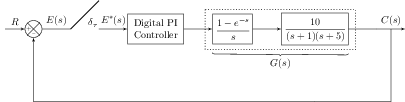
\includegraphics[width=1\linewidth]{Diagrams/block410.pdf}
	\caption*{Figure 4-68}
	\label{fig:samplerblock413}
\end{figure}
Let the PI controller be $\displaystyle G_{PI}(z)=K_p+K_i\frac{1}{1-z^{-1}}=(K_p+K_i)\cfrac{z-\frac{K_p}{K_p-K_i}}{z-1}$ and discretizing $G(s)$
\begin{align*}
& G_{PI}(z)G(z)=G_{PI}(z)\frac{\frac{13711\,z}{100000}+\frac{46027827}{500000000}}{\left(z-\frac{3679}{10000}\right)\,\left(z-\frac{8187}{10000}\right)}=(K_p+K_i)\cfrac{z-\frac{K_p}{K_p-K_i}}{z-1}\frac{0.13711\,z+0.092055654}{\left(z-0.3679\right)\,\left(z-0.8187\right)} \\
& \text{Pick } \frac{\omega_d}{\omega_s}=0.1, \quad \text{since } \zeta=0.5, |z| = \exp \left(\frac{-2\pi \zeta}{\sqrt{1-\zeta^2}}\frac{\omega_d}{\omega_s} \right)=0.6958 \quad \angle z = \frac{360^\circ}{10}= 36^\circ %, z=0.5629 + j0.4090
\end{align*}

% Since the description will be commented out in the final version, could use if package to automatic this process.
\begin{figure}[H]
	\centering
	\includegraphics[width=1\linewidth]{Diagrams/poleszeroes.pdf}
	\caption{Diagram illustrating that the zero $z-\frac{K_p}{K_p-K_i}$ must contribute $125.1015^\circ$}
	\label{fig:polesZeroess}
\end{figure}

\begin{align*}
& \angle \left.\left(z-\frac{K_p}{K_p-K_i}\right)\right\vert_{z=0.5629 +j0.4090} = 125.1015^\circ \quad \cfrac{0.409}{0.5629-\frac{K_p}{K_p-K_i}} = \tan(125.1015^\circ)
\end{align*}
\begin{align}
&
\frac{K_p}{K_p-K_i}= 0.850366 \label{eq:kipi1} \\
\notag & (K_p+K_i)\left|\frac{\left(z+0.6714\right)\,\left(0.13711\,z-0.028038995\right)}{(z-0.3679)\,(z-0.8187)}\right|_{z=0.5629 +j0.4090}=1 \\ 
&
0.44357786197\,K_i+0.44357786197\,K_p=1.0 \label{eq:kipi2} 
\end{align}

Solving \eqref{eq:kipi1} and \eqref{eq:kipi2} leads to $K_i=0.33733$ and $K_p=1.9171$.

\[
G_{PI}G(z)=2.254396\cfrac{z-0.850366}{z-1}\frac{0.13711\,(z+0.6714)}{\left(z-0.3679\right)\,\left(z-0.8187\right)}
\]
\begin{align*}
& K_v = \lim\limits_{z \rightarrow 1} \frac{z-1}{z \ T} G_{PI}G(z) = \frac{1}{0.2(1)} \frac{0.149634(0.13711(1.6714))}{(0.6321)(0.1813)}=1.496119
\end{align*}
\subsubsection*{Problem B-4-15}
Using the Bode diagram approach in the $w$ plane, design a digital controller for the system shown in Figure 4-72. The design specifications are that the phase margin be $50^\circ$, the gain margin be at least 10 dB, and the static velocity error constant $K_v$ be 20 $\text{sec}^{-1}$. The sampling period is assumed to be 0.1 sec, or $T = 0.1$. After the controller is designed, calculate the number of samples per cycle of damped sinusoidal oscillation.

\begin{figure}[H]
	\centering
	\includegraphics[width=1\linewidth]{Diagrams/block415.pdf}
	\caption*{Figure 4-72}
	\label{fig:samplerblock415}
\end{figure}

\begin{align*}
& G(z) = \mathcal{Z} \left[\frac{1-e^{-sT}}{s}\frac{K}{s(s+0.5)}\right]=0.004918K \frac{z+0.9835}{(z-1)(z-0.9512)}
\end{align*}

Running the \lstinline[language=Matlab]|ass_5.m| in Matlab as with the parameters specified in \textbf{ass\_5.out} results in:
\[
\frac{0.32774 z^3 - 0.27218 z^2 - 0.31605 z + 0.26423}{z^4 - 2.7603 z^3 + 2.3775 z^2 - 0.47208 z - 0.14507}
\]
\begin{figure}
	\centering
	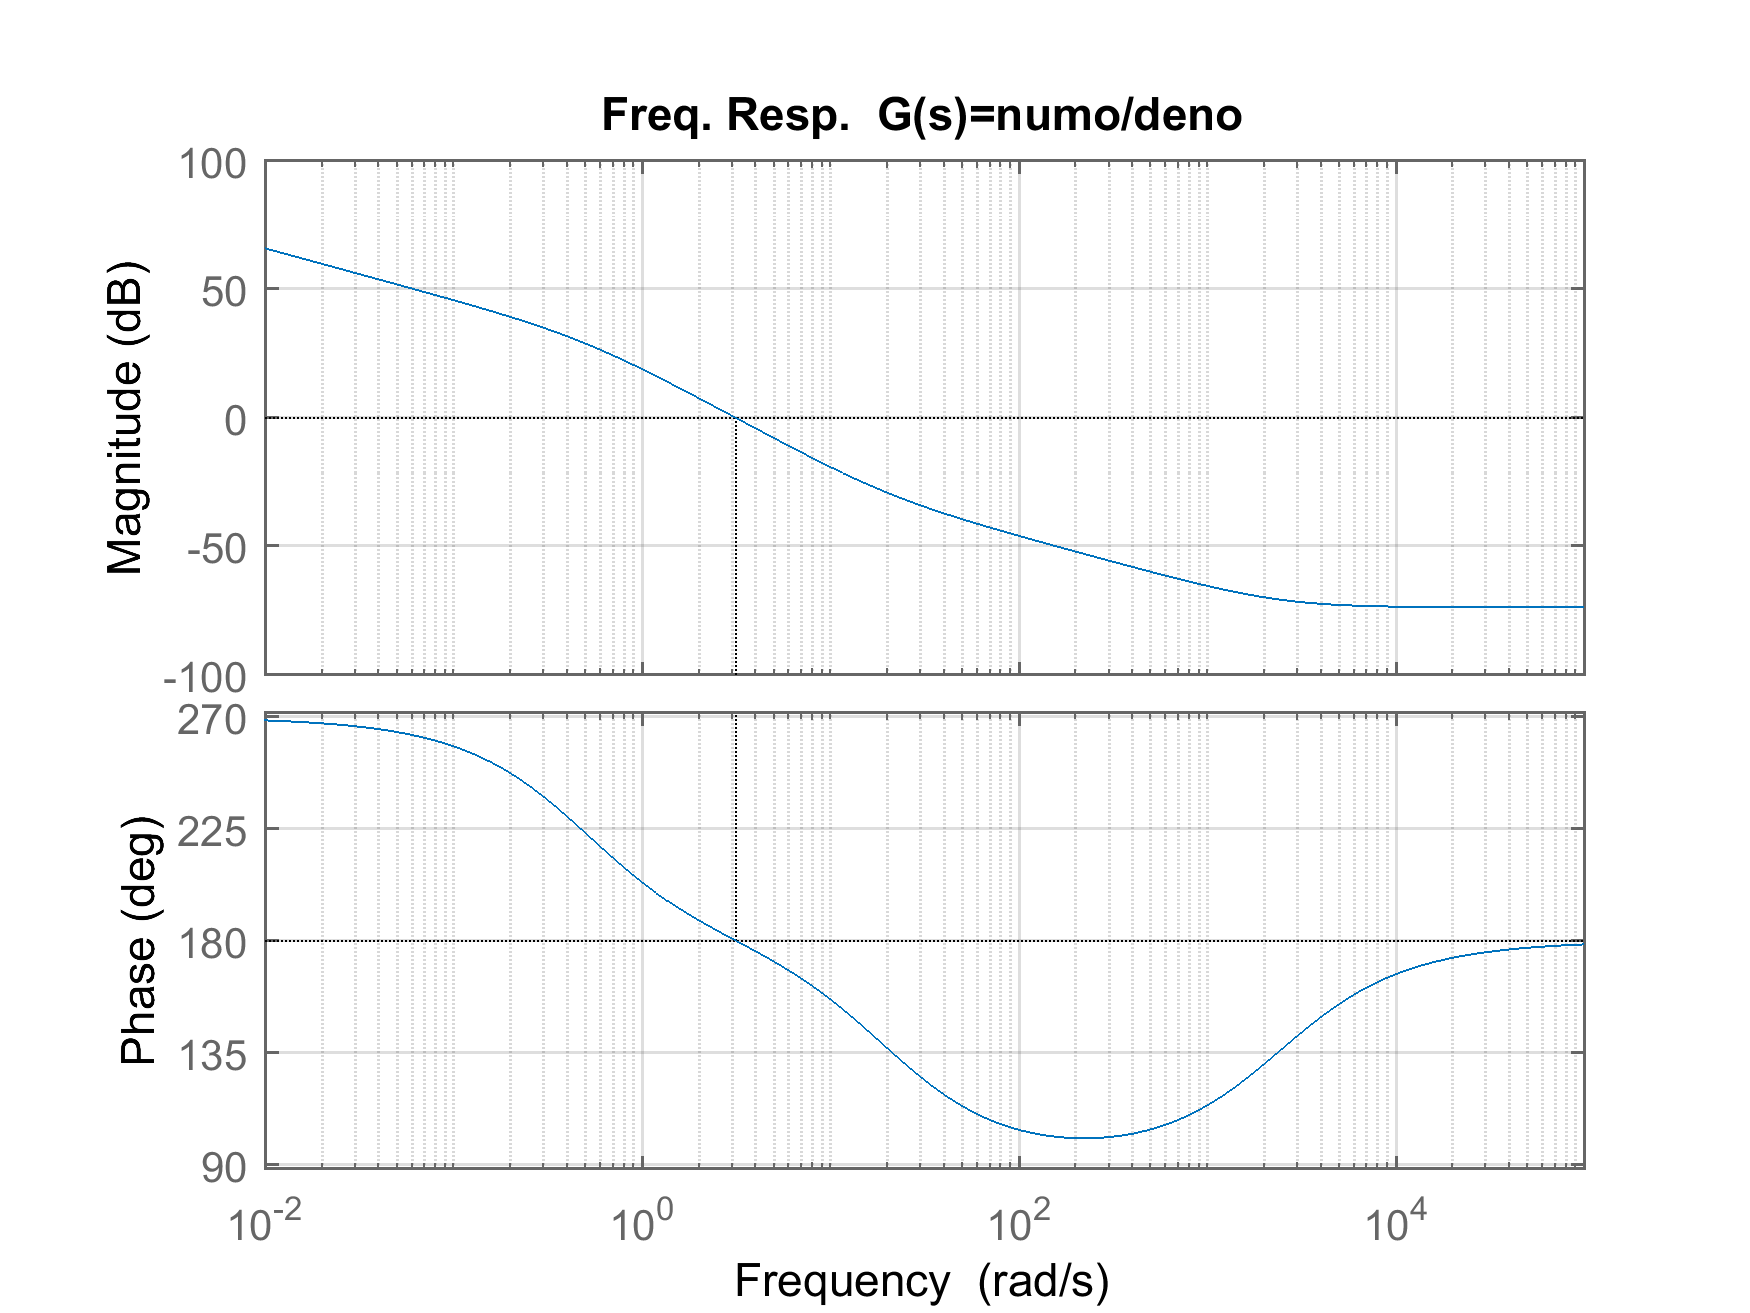
\includegraphics[width=0.6\linewidth]{MatlabPlots/bodePlotUnComp.png}
	\caption{Bode Plot for uncompensated System}
	\label{fig:bodePlotUnComp}
\end{figure}

\begin{figure}
	\centering
	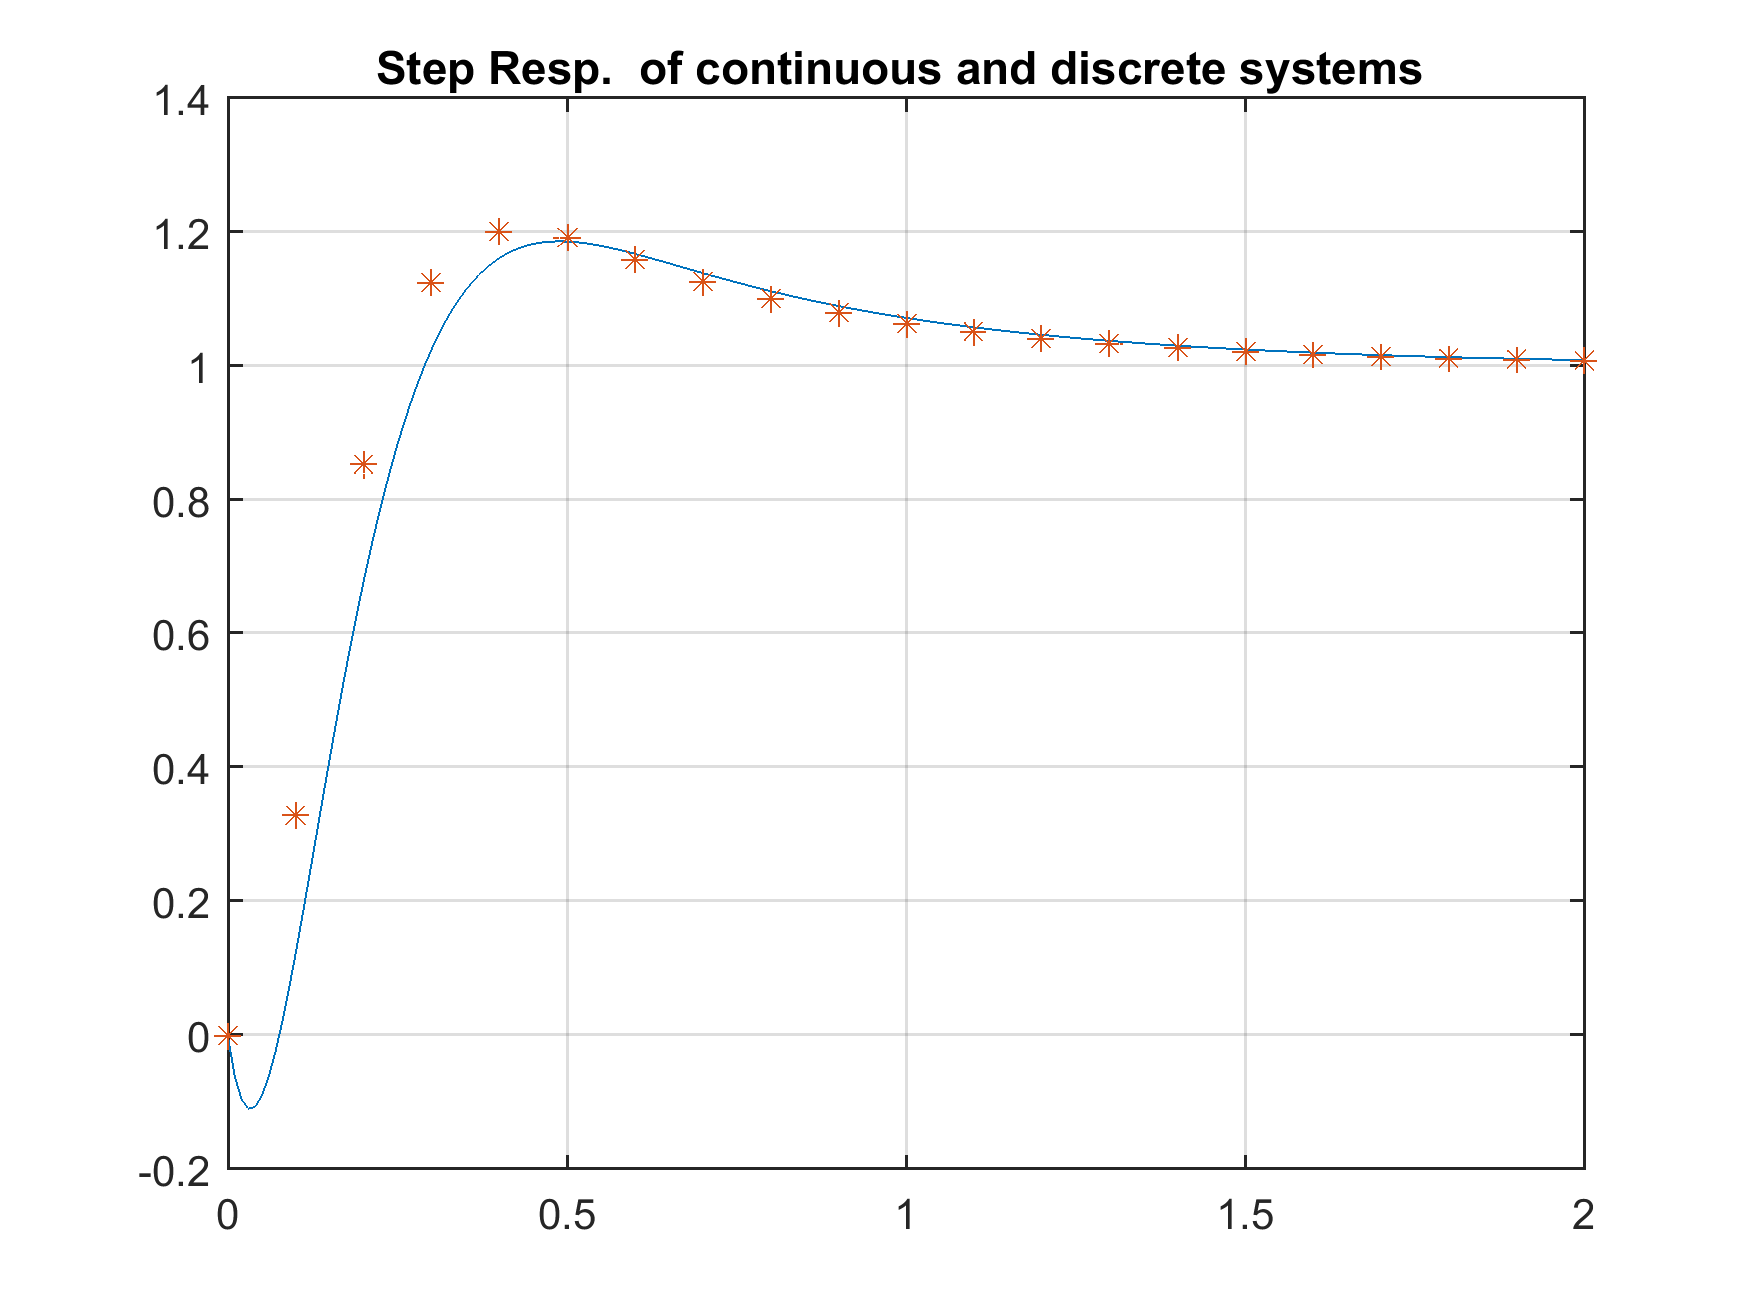
\includegraphics[width=0.6\linewidth]{MatlabPlots/stepRespCTSDS.png}
	\caption{Bode Plot for uncompensated System}
	\label{fig:Step Response}
\end{figure}
\begin{lstlisting}[language=Matlab]
Discrete Compensator): 

num/den = 

66.6418 z^2 - 120.8858 z + 54.6277
----------------------------------
z^2 - 0.80914 z - 0.15251
Open loop compensated discrete system transfer function

num/den = 

0.32774 z^3 - 0.27218 z^2 - 0.31605 z + 0.26423
---------------------------------------------------
z^4 - 2.7603 z^3 + 2.3775 z^2 - 0.47208 z - 0.14507
Closed loop zeros and poles of discrete system
zeros =
	-0.9835
	0.9608
	0.8532
poles =
	0.9607 + 0.0000i
	0.8039 + 0.0000i
	0.3340 + 0.2068i
	0.3340 - 0.2068i
Number of samples per cycle:
ans =
11.3339
\end{lstlisting}